\documentclass{article}

\usepackage{listings}
\usepackage{todonotes}
\usepackage{verbatim}
\usepackage{tikz}
\usepackage{tkz-graph}
\usepackage{pgf}
\usetikzlibrary{arrows,automata}

% \newcommand*\beastscriptr{\verb;beastscriptr;}

\title{beastscriptr: BEAUti for R}
\author{Rich\`el J.C. Bilderbeek}


% \newcommand*\filename[1]{${#1}$}
% \newcommand*\myfilename[1]{\verb;{#1};}

% Style of code
% From http://r.789695.n4.nabble.com/How-to-nicely-display-R-code-with-the-LaTeX-package-listings-tp4648110.html
\usepackage{fancyvrb} 
\definecolor{codegreen}{rgb}{0,0.6,0}
\definecolor{codegray}{rgb}{0.5,0.5,0.5}
\definecolor{codepurple}{rgb}{0.58,0,0.82}
\definecolor{backcolour}{rgb}{0.95,0.95,0.92}
\lstdefinestyle{mystyle}{
  language=R,% set programming language
  basicstyle=\ttfamily\small,% basic font style
  commentstyle=\color{gray},% comment style
  numbers=left,% display line numbers on the left side
  numberstyle=\scriptsize,% use small line numbers
  numbersep=10pt,% space between line numbers and code
  tabsize=2,% sizes of tabs
  showstringspaces=false,% do not replace spaces in strings by a certain character
  captionpos=b,% positioning of the caption below
  breaklines=true,% automatic line breaking
  escapeinside={(*}{*)},% escaping to LaTeX
  fancyvrb=true,% verbatim code is typset by listings
  extendedchars=false,% prohibit extended chars (chars of codes 128--255)
  literate={"}{{\texttt{"}}}1{<-}{{$\bm\leftarrow$}}1{<<-}{{$\bm\twoheadleftarrow$}}1
  {~}{{$\bm\sim$}}1{<=}{{$\bm\le$}}1{>=}{{$\bm\ge$}}1{!=}{{$\bm\neq$}}1{^}{{$^{\bm\wedge}$}}1,% item to replace, text, length of chars
  alsoletter={.<-},% becomes a letter
  alsoother={$},% becomes other
  otherkeywords={!=, ~, $, \&, \%/\%, \%*\%, \%\%, <-, <<-, /},% other keywords
  deletekeywords={c}% remove keywords 
}
\lstset{style=mystyle}

\begin{document}

\maketitle

\begin{abstract}
  \textbf{1. }
  Here, I present a package, \verb;beastscriptr;, for the R programming language. \\
  \textbf{2. }
    \verb;beastscriptr; allows for scripted use of the BEAST2 phylogenetics tool, 
    by creating BEAST2 input files from an R function call. \\
  \textbf{3. }
    I describe \verb;beastscriptr; usage, the novel functionality it provides
    compared to BEAUti, and give some minimal examples. \\
  \textbf{4. }
    As \verb;beastscriptr; is free, libre, open-source and designed to be extended, 
    I conclude by describing the current development of the package \\
\end{abstract}

% Key-words: computational biology, evolution, phylogeny, BEAST2, R

%%%%%%%%%%%%%%%%%%%%%%%%%%%%%%%%%%%%%%%%%%%%%%%%%%%%%%%%%%%%%%%%%%%%%%%%%%%%%%%%%%%%%%
\section{Introduction}
%%%%%%%%%%%%%%%%%%%%%%%%%%%%%%%%%%%%%%%%%%%%%%%%%%%%%%%%%%%%%%%%%%%%%%%%%%%%%%%%%%%%%%

BEAST2 \cite{bouckaert2014beast} is a popular Bayesian phylogenetics tool.
BEAST2 is bundled with the program called BEAUti \cite{drummond2012bayesian},
which  allows for a user-friendly way to create the
input files that BEAST2 needs. BEAUti is convenient to get started, yet
does not allow for the scripted use of BEAST2. For creating BEAST2 input
files from a script, beastscriptr is the R package facilitating this:
it creates a BEAST2 input files from an R function call.

%\begin{figure}
%  \centering
%  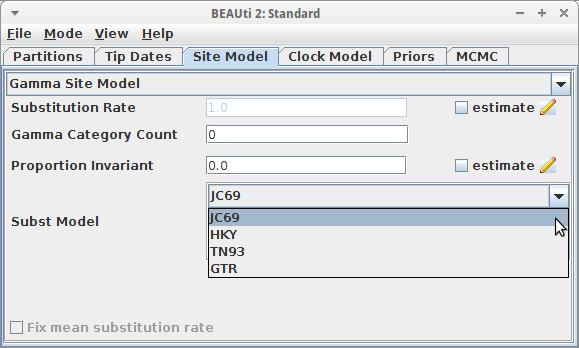
\includegraphics[]{BeautiSiteModel.png}
%  \caption{BEAUti}
%  \label{figure:beauti}
%\end{figure}

%%%%%%%%%%%%%%%%%%%%%%%%%%%%%%%%%%%%%%%%%%%%%%%%%%%%%%%%%%%%%%%%%%%%%%%%%%%%%%%%
\begin{figure}
  \centering
  \begin{tikzpicture}[->,>=stealth',shorten >=1pt,auto,node distance=6cm, semithick]   
  \tikzstyle{every state}=[]
  \node[state] (A) [rectangle] {
    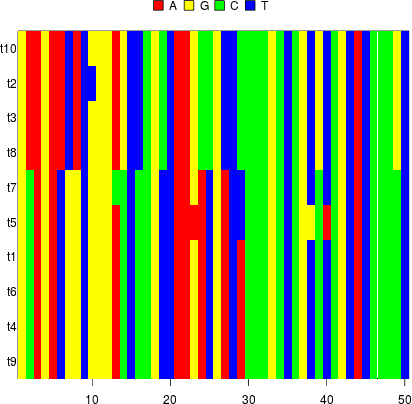
\includegraphics[width=0.2\textwidth]{alignment.png}
    
\includegraphics[width=0.2\textwidth]{thought_cloud.png}
  };   
  \node[state] (E) [below of=A, rectangle] {
    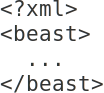
\includegraphics[height=0.1\textheight]{xml.png}
  };   
  \node[state] (F) [rectangle, below of=E] {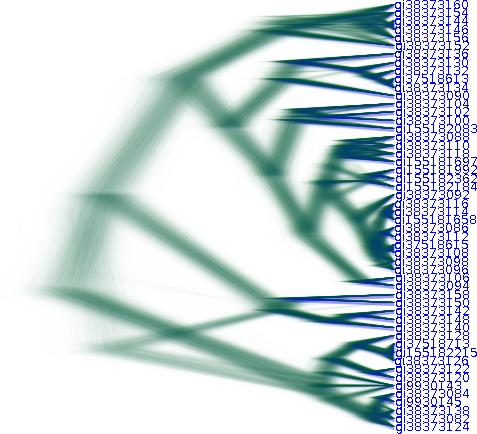
\includegraphics[width=0.3\textwidth]{DensiTreeExample2.jpg}};
  \path (A) edge [anchor = east] node {
\includegraphics[height=0.15\textheight]{beastscriptr_logo.png}} (E)
        (A) edge [anchor = west] node {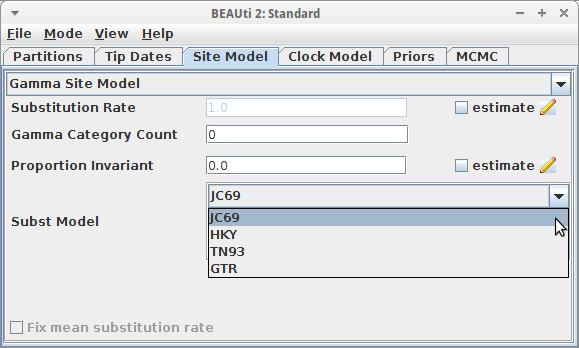
\includegraphics[height=0.15\textheight]{BeautiSiteModel.png}} (E)
        (E) edge [] node {
\includegraphics[width=0.2\textwidth]{Beast2LogoRat.png}} (F); 
  \end{tikzpicture}

  \caption{
    Workflow. From an alignment and priors, one creates a BEAST2 XML input file. This
    can be done using beastscript and BEAUti. The XML file created is run by BEAST2
    to create a posterior.
  }
  \label{fig:workflow}
\end{figure}
%%%%%%%%%%%%%%%%%%%%%%%%%%%%%%%%%%%%%%%%%%%%%%%%%%%%%%%%%%%%%%%%%%%%%%%%%%%%%%%%

%%%%%%%%%%%%%%%%%%%%%%%%%%%%%%%%%%%%%%%%%%%%%%%%%%%%%%%%%%%%%%%%%%%%%%%%%%%%%%%%%%%%%%
\section{Descriptions}
%%%%%%%%%%%%%%%%%%%%%%%%%%%%%%%%%%%%%%%%%%%%%%%%%%%%%%%%%%%%%%%%%%%%%%%%%%%%%%%%%%%%%%

The goal of the R package \verb;beastscriptr; is to create the 
same BEAST2 input files that BEAUti creates, but from one R function call 
instead.

By creating BEAST2 input files in BEAUti, 
the desired output of beastscriptr was determined. 
The functionality of BEAUti is added gradually (and is still growing).

\verb;beastscriptr; has only parts of the functionality of BEAUti, yet
can be extended easily. beastcriptr, on the other hand, does allow for specifying
to use phylogenies of fixed crown age.

\verb;beastscriptr; has a novel functionality not built into BEAUti yet:
it allows for using phylogenies of a fixed crown age. 


%%%%%%%%%%%%%%%%%%%%%%%%%%%%%%%%%%%%%%%%%%%%%%%%%%%%%%%%%%%%%%%%%%%%%%%%%%%%%%%%%%%%%%
\section{Examples}
%%%%%%%%%%%%%%%%%%%%%%%%%%%%%%%%%%%%%%%%%%%%%%%%%%%%%%%%%%%%%%%%%%%%%%%%%%%%%%%%%%%%%%

As in BEAUti, to create a BEAST2 input file, 
one needs an alignment and model settings.
With those settings at their default, \verb;beastscriptr; is easy to use:
Create a BEAST2 input file with name \verb;beast2.xml; from 
a FASTA file with name \verb;alignment.fas; is done like this:

\begin{lstlisting}[language=R, caption=Simplest example]
library(beastscriptr)
create_beast2_input_file(
  "alignment.fas",
  "beast2.xml"
)
\end{lstlisting}

The created file \verb;beast2.xml; can then be used by BEAST2.

Novel about beastscriptr is that it allows for specifying a fixed crown age:

\begin{lstlisting}[language=R, caption=Example with fixed crown age]
create_beast2_input_file(
  "alignment.fas",
  "beast2.xml"
  fixed_crown_age = TRUE,
  initial_phylogeny = beastscriptr::fasta_to_phylo(
    fasta_filename = "alignment.fas", 
    crown_age = 15
  )
)
\end{lstlisting}

In this example, a random phylogeny is created from the FASTA file, but
one could also use a more informed initial phylogeny with the desired crown age. 

%%%%%%%%%%%%%%%%%%%%%%%%%%%%%%%%%%%%%%%%%%%%%%%%%%%%%%%%%%%%%%%%%%%%%%%%%%%%%%%%%%%%%%
\section{beastscriptr development and other resources}
%%%%%%%%%%%%%%%%%%%%%%%%%%%%%%%%%%%%%%%%%%%%%%%%%%%%%%%%%%%%%%%%%%%%%%%%%%%%%%%%%%%%%%

beastscriptr successfully creates valid BEAST2 input files. Unlike BEAUti,
beascriptr allows for setting a fixed crown age.

beastscriptr does not support the full functionality of BEAUti. Considering
the size, age and number of plugins, this would be close to impossible.
To compensate for this, an extensible software architecture is used.

beastscriptr has minimal support for calling BEAST2 from within R and does
so for testing purposes. 

beastscript has minimal support for parsing and interpreting BEAST2 output files,
for that the RBeast package is recommended.

The package is free and is available from the official R package archive at 
http://cran.r-project.org/src/contrib/PACKAGES.html\#beastscriptr. 
beastscriptr is licensed under the GNU General Public License.


%%%%%%%%%%%%%%%%%%%%%%%%%%%%%%%%%%%%%%%%%%%%%%%%%%%%%%%%%%%%%%%%%%%%%%%%%%%%%%%%%%%%%%
\section{Citation of beastscriptr}
%%%%%%%%%%%%%%%%%%%%%%%%%%%%%%%%%%%%%%%%%%%%%%%%%%%%%%%%%%%%%%%%%%%%%%%%%%%%%%%%%%%%%%

Scientists using beastscriptr in a published paper should cite this
article. Users can additionally cite the beastscriptr package 
directly. Citation information can be obtained by typing:

\begin{lstlisting}[language=R]
> citation("beastscriptr")
\end{lstlisting}

from within R.

%%%%%%%%%%%%%%%%%%%%%%%%%%%%%%%%%%%%%%%%%%%%%%%%%%%%%%%%%%%%%%%%%%%%%%%%%%%%%%%%%%%%%%
\section*{Acknowledgements}
%%%%%%%%%%%%%%%%%%%%%%%%%%%%%%%%%%%%%%%%%%%%%%%%%%%%%%%%%%%%%%%%%%%%%%%%%%%%%%%%%%%%%%

We would like to thank the Center for Information Technology of the University of Groningen for their support
and for providing access to the Peregrine high performance computing cluster.

%%%%%%%%%%%%%%%%%%%%%%%%%%%%%%%%%%%%%%%%%%%%%%%%%%%%%%%%%%%%%%%%%%%%%%%%%%%%%%%%%%%%%%
\bibliographystyle{plain}
\bibliography{article}

\begin{thebibliography}{}

\end{thebibliography}
%%%%%%%%%%%%%%%%%%%%%%%%%%%%%%%%%%%%%%%%%%%%%%%%%%%%%%%%%%%%%%%%%%%%%%%%%%%%%%%%%%%%%%

\end{document}
